\section{Stability and Performance Analysis}

\subsection{Basic System Classes}

\subsubsection{First Order Systems}
State-space representation of first order system:
$$\dot{x} = -\frac{1}{\tau}x+\frac{k}{\tau}u$$
$$y=x$$

A first-order system has one  pole and is described by:
$$H(s)=\frac{k}{\tau s+1}$$
Where \emph{k} is the DC-gain and $\tau$ is the time-constant. The system has a pole
in $s=-\frac{1}{\tau}$ i.e., the smaller time-constant, the faster system response.


\subsubsection{Second Order Systems}
The transfer funciton of a second-order system is given by:
$$H(s) = \frac{k \omega_n^2}{s^2+2\zeta\omega_n s+\omega_n^2}$$
Where $\omega_n>0$ is the natural frequency and $\zeta>0$ is the damping ratio and k is the gain.

The system has two poles, which are $s\in \mathbb{C}$ where:
$$s^2+2\zeta\omega_n s+\omega_n^2=0$$
The values of s is given by:
$$s = -\zeta\omega_n \pm j\omega_n\sqrt{1-\zeta^2}$$

When $\zeta=1$ the system is critically damped and $H(s)$ has a double pole in $s=-\zeta \omega_n$,
when $0<\zeta<1$ the system is underdamped and has complex poles.
When $\zeta>1$ the system is overdamped and has real and distinct poles.

\begin{center}
	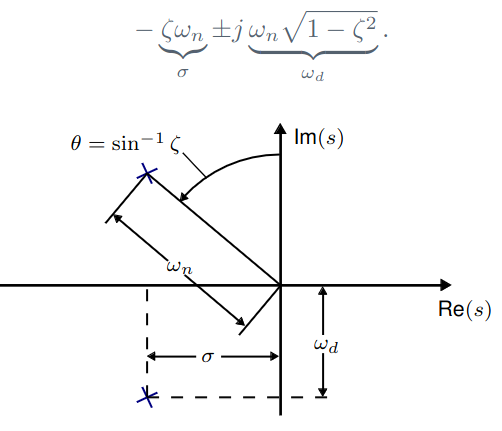
\includegraphics[width=0.5\textwidth]{Images/secondOrderSystem.png}
\end{center}

\subsection{Performance specifications}
\subsection{Stability}
The stability of the dynamical system can be determined from the eigenvalues of A in the time domain.
$$\dot{x} = Ax+Bu$$
$$y=Cx+Du$$

When the eigenvalues of A are in the left half plane, the system is stable.


In the frequency domain the stability can be determined from the poles of G(s) seen from the transfer function:
$$G(s) = \frac{Q(s)}{P(s)}$$

When the poles of G(s) are in the left half plane, the system is stable.



\subsection{Examples}
